

\begin{lstlisting}[language=Python]
def function_3(img):
    res = img.copy()
    for i in range(1, img.shape[0] - 1):
        for j in range(1, img.shape[1] - 1):
            up = (img[i, j] != img[i + 1, j]).any()
            down = (img[i, j] != img[i - 1, j]).any()
            left = (img[i, j] != img[i, j - 1]).any()
            right = (img[i, j] != img[i, j + 1]).any()
            if up or down or left or right:
                res[i, j] = np.array([0, 0, 0])  # Cor preta
    return res

# Aplicacao do algoritmo
output = function_1(imagem, 4)
edge = function_3(output)
\end{lstlisting}

\begin{figure}[H]
    \centering
    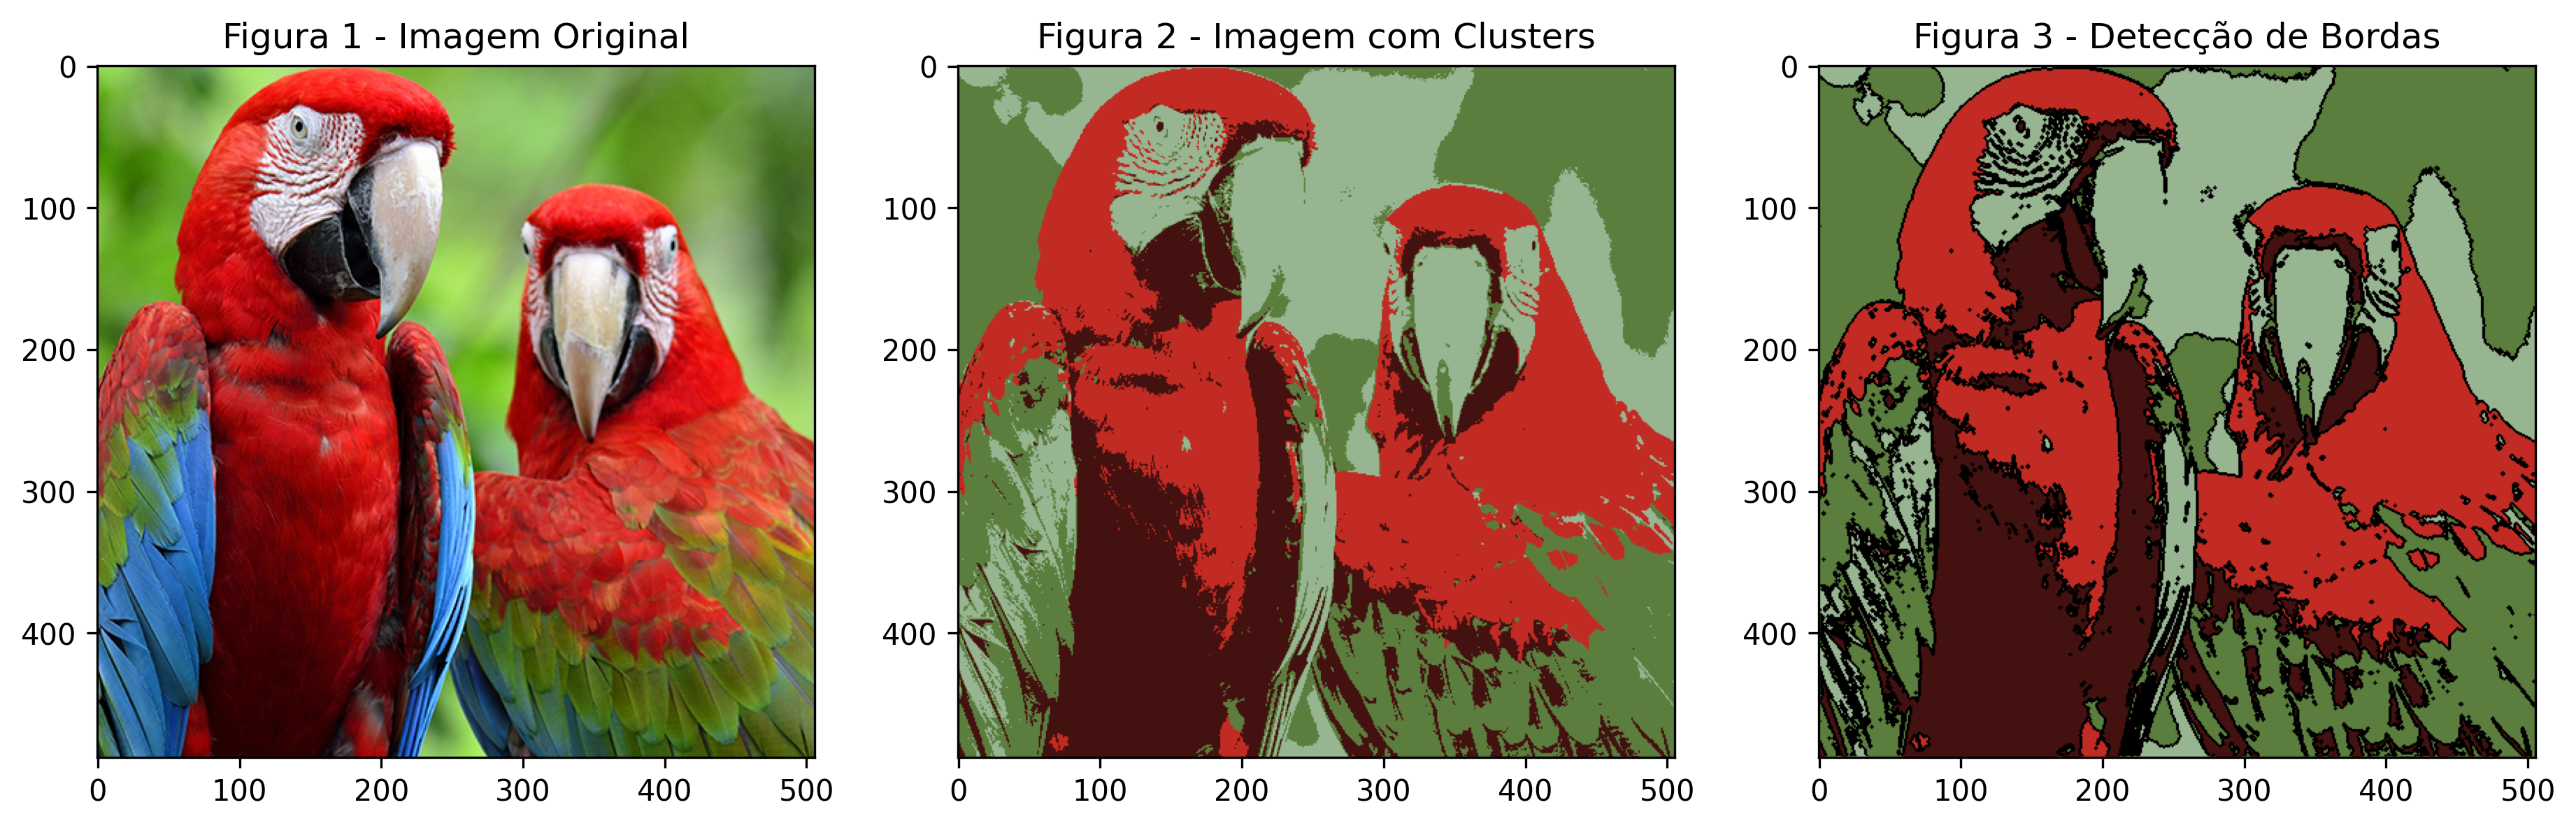
\includegraphics[width=0.9\textwidth]{../figures/5/edge_detection.png}
    \caption{Algoritmo de detecção de bordas baseado em clustering}
    \label{fig:edge_detection}
\end{figure}